


\section{Aims \& Objectives}
\subsection{Aims}

The aim of the project is to create one of these BZ simulations and add a number of imperfections, measuring how they impact the simulation. These imperfections would typically be found in the real world in the form of dust particles, terrain obstacles or other environmental factors.
\begin{figure}
    \centering
    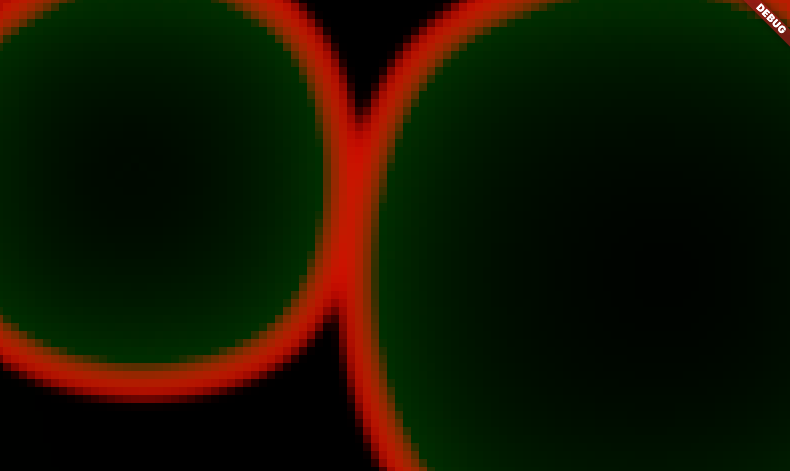
\includegraphics[width=0.75\linewidth]{original_proposal/Screenshot 2023-10-24 at 08.09.52.png}
    \caption{Expanding wave pattern from this project using the Oregonator model}
    \label{fig:first-waves}
\end{figure}

The main idea is to create an application using Flutter and to simulate the reaction. 
\begin{enumerate}
    \item Interactive Simulation App Development with Flutter
    Flutter is a mobile application framework that allows for easy addition of elements of interactivity and allows for lower level control over pixels, which is necessary for creating one of these simulations. The reason for choosing Flutter as opposed to another framework or solution is because of the already present familiarity with the framework. 

    The simulation shall run on the GPU, so addressing the GPU usage is crucial. The current solutions are to use the recently added \verb|flutter_gpu| package or integrating Dart Foreign Function Interface (FFI) to run native shaders. 
    \item Creating a game from the simulation. Since the project is focused around imperfections, it could be possible to let the user play with or against the waves (see figure \ref{fig:enter-label}) using the \verb|flame| package (minimal game engine). 

    The simulation has illumination that creates a path, the aim is to create a game where the user has to run away from the waves, but is also constrained to the illuminated area, so for example a single wave could split and then catch the player from both directions. 

    \item Adding imperfections:
    One of the main themes of the project is finding imperfections. The goal is to let the player defend himself from the waves using imperfections in the simulation that impact the reaction-diffusion model. This could mean throwing dust particles at the wave or adding temperature to the model that speeds up or slows down the reaction at a particular zone, so that a part of the waves travels more slowly, disrupting the reaction. The aim is to allow the user to only use imperfections as a means of defence. 
\end{enumerate}

\subsection{Challenges}
Among the challenges I might face I see myself running into a computational problem where dt, being as small as it is, could force me to run the simulation at a very slow rate, which then would make me increase the speed at which it is run, using more CPU, but since the project is \textit{real time}, I cannot afford to go beyond the maximum allowed CPU per frame or I would cause jitter, running code on the GPU should help, but there also needs to be a way to only perform these calculations on a subset of the whole map. Also if this were a game, there could be beacons generating these waves that the user has to destroy. Flutter also has a 2D game engine that I've wanted to explore and that could be a great opportunity. 
The other reaction-diffusion systems are very scientific or are presented as a video. \cite{doi:10.1021/jp509474w} have used reaction and diffusion to find the shortest path in a maze. 

\section{Related work}
The area of reaction-diffusion simulations has been explored well. The simulations of waves are used to produce computing units like counters and logic gates \citep{gorecki2003chemical} as well as neurons \citep{StovoldJames2019RaGI}. 

\cite{edge2020chaotic} has created a game (figure \ref{fig:chaotic-edge-game}) out of the Gray-Scott model where ships battle inside of a goo-like substance and the chemical acts as a dynamic obstacle. The game looks of very high quality despite the lack of interest from the public. Other than this project, there isn't a lot of interest in the joint field of reaction-diffusion simulations and gaming
\begin{figure}
    \centering
    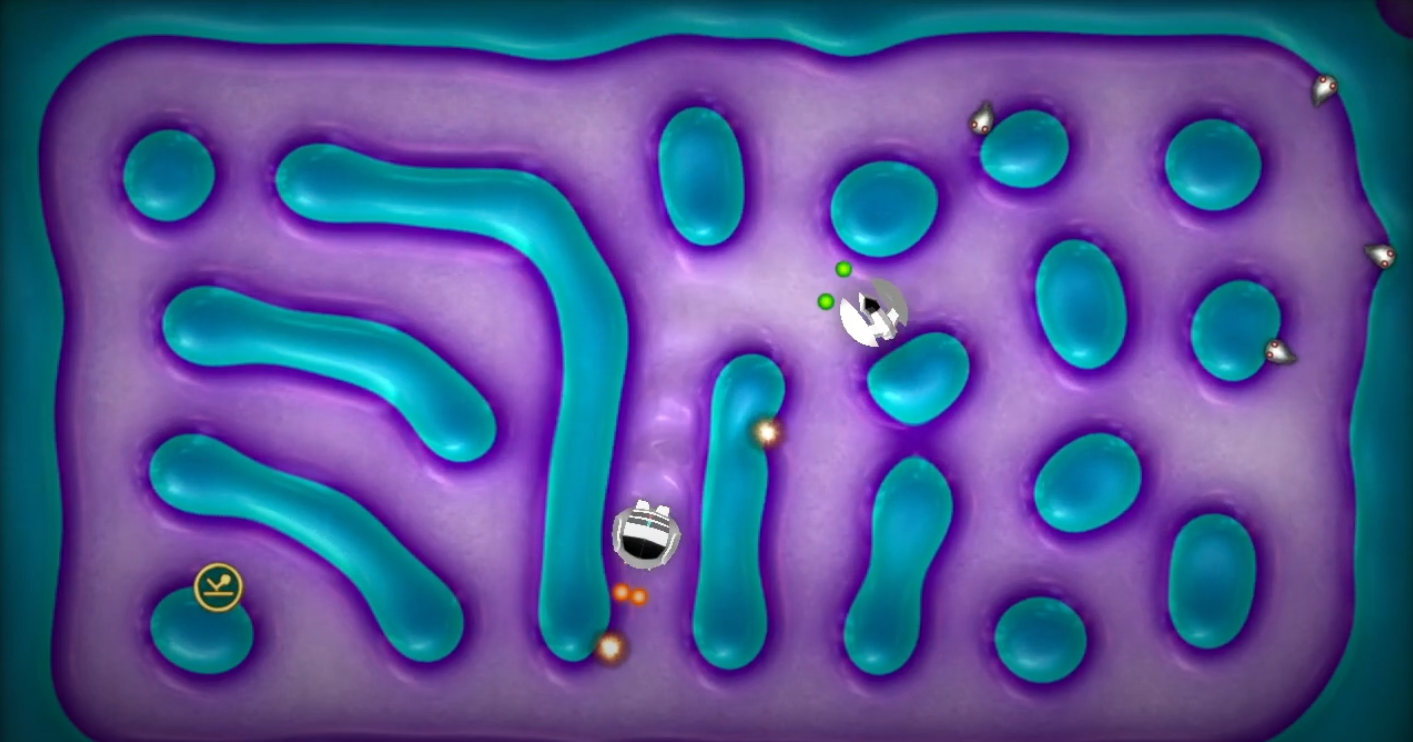
\includegraphics[width=0.75\linewidth]{original_proposal/Screenshot 2023-10-26 at 06.06.23 (1).png}
    \caption{Reaction Diffusion Game by Chaotic Edge}
    \label{fig:chaotic-edge-game}
\end{figure}
\section{Methodologies}
\begin{enumerate}
    \item The project is going to use an agile iterative approach where the phases of the Software Development Life Cycle are performed every sprint.

    \item It's important is that the work is broken down into chunks according to the SMART task framework, which stands for Specific, Manageable, Achievable, Relevant, Time-bound. It's important for the tasks to be small and understandable, without any dependencies to other tasks
    \item If one task requires the parallel completion of another task, then these tasks should be the same task with two things to do in the task. 
    \item The project is going to use ClickUp as a Project Managemenet System (PMS) due to its flexibility and integration with calendar and task management apps. 
    \item The most important task management tool to be used in this project is Reclaim.AI, which uses priorities and deadlines to auto schedule your calendar based on your preferences and hours, it has an integration with the most popular PMSs like Jira, ClickUp, Asana, etc. 
    \item The Project Management System tasks are going to use custom statuses:
    \begin{enumerate}
        \item TODO - feature not started
        \item RESEARCHING - gathering information and reading about feature
        \item SUBTASKING - feature clear. creating subtasks and checklists to make task execution easier
        \item IMPLEMENTING - implementing feature
        \item TO PRESENT - feature implemented. Waiting to be presented to supervisor
        \item FOR REVISION - supervisor left feedback. Return task to RESEARCHING or IMPLEMENTING
    \end{enumerate}
    \item The project is going to use the 1 week sprints to divide work into even blocks of work if the backlog ends up being too big. If the backlog remains small , the project is going to use the backlog and not use sprints. 
\end{enumerate}
\section{Programme of Work}
The project, being agile, doesn't have strong formal phases, it follows an iterative approach. 
There are however distinct phases in the planned development of this project (see figure \ref{fig:gantt}):

\begin{enumerate}
    \item Planning \& Analysis - this phase is going to specify goals of the sprint
    \item Design - The project is going to be designed in more detail, that includes library choices, design choices, etc
    \item Implementation - This phase would take up the majority of the sprint time
    \item Testing - last phase before the project transitions into a finalising state
    \item Searching for Participants - a stage where about 5 people need to be recruited to perform evaluation
    \item Conduct evaluation - the evaluation is going to be performed using heuristics, for example how intuitive the game is, etc. 
    \item Focus on dissertation - time to shift focus on using the resources and documentation to create the dissertation.
\end{enumerate}
This project is prototypical, so it's going to have reduced planning and design phases. 
\begin{figure}
    \centering
    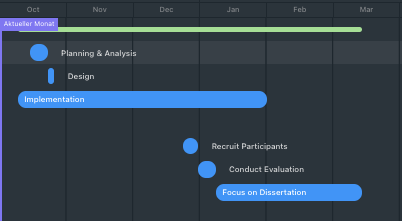
\includegraphics[width=1\linewidth]{original_proposal/Screenshot 2023-10-26 at 18.26.29.png}
    \caption{Gantt Chart}
    \label{fig:gantt}
\end{figure}
